\chapter{Revisão Bibliográfica} \label{chap:sota}

\section{Introdução}

Neste capítulo são analisadas todas as áreas científicas relevantes
para que esta dissertação possa ser realizada com sucesso, tirando partido do
conhecimento mais avançado do que está a ser feito a nível mundial e até 
equacionar novas abordagens para melhorar as soluções existentes para o problema
do reconhecimento de objectos. Mais particularmente o que está feito em termos de
reconhecimento de objectos 3D em termos ciêntíficos e das bibliotecas existentes
nesse âmbito.

Faz-se também uma análise ao que existe em termos de demonstradores de robótica autónoma
para enquadrar o trabalho a ser desenvolvido respeitante à utilização dos objectos,
que sendo reconhecidos como marcadores influenciam o comportamento do robô.

\section{Sistemas de Percepção para reconhecimento de Objetos}

\subsection{Time of Flight Camera}

Esta câmara tem receptores para obter o tempo de vôo (i.e.: time-of-flight)
de uma partícula de luz de modo a saber a que distância se encontram os
obstáculos no campo de visão da câmara. Existem várias implementações desta
tecnologia, mas a mais usual é ter um emissor de luz, por norma um laser,
que envia pulsos de luz que são reflectidos nos obstáculos e são captados por
um sensor que a cada “pixel” recebe a distância a que o objecto se encontra.

É um sensor que tem muitas aplicações, entre as quais a detecção de objectos nas imediações
pois permite obter distâncias dos objectos que se encontram no seu campo
de visão sem que isso implique um maior custo de cálculo através de algoritmos
de visão por computador. 

\subsection[LIDAR]{Light Detection and Ranging}

Os sistemas LIDAR utilizam um feixe de luz rotativo para fazer mapeamento 3D
do ambiente que o circunda. A vantagem destes sistemas é que, com feixes de
luz muito estreitos conseguem obter uma resolução muito grande, sendo o ideal
para aplicações críticas, tais como o alunar de sondas no caso da NASA \cite{Keim2010}.

Os LIDAR utilizam técnicas de \emph{backscattering} para conseguir uma medição
precisa de distância (além de algumas características do alvo), sendo necessário
fazer algumas considerações prévias sobre o meio em que se vai propagar o laser
para escolher o melhor comprimento de onda.


\subsection{Kinect}
O \emph{Kinect} é um sensor 3D desenvolvido pela \emph{Microsoft}, cujo objectivo principal era
ser utilizado a par com o sistema X-Box 360, para a interacção com jogos sem recorrer
a controladores, sendo que através deste sensor os movimentos do jogador controlam o
jogo. Este foi o primeiro sensor 3D disponível para o utilizador comum e massificou o
acesso da comunidade ciêntífica a este tipo de sensores, que de outra forma seriam
demasiado dispendiosos.

As aplicações deste sensor fora do âmbito original para que foi desenvolvido são inúmeras,
e rapidamente foi desenvolvido um controlador \emph{opensource} para se desenvolver aplicações
em qualquer sistema operativo.

\begin{center}
	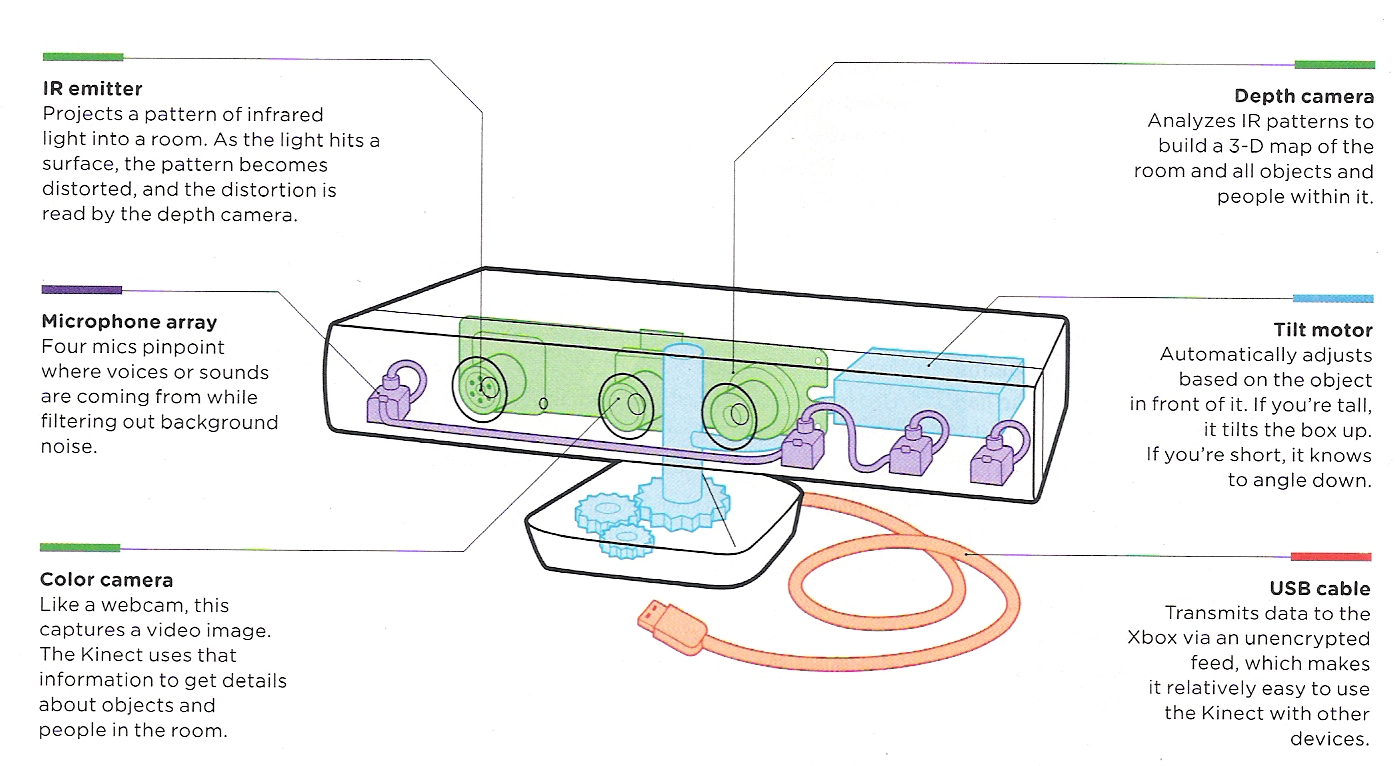
\includegraphics[width=0.80\textwidth]{figures/Kinect.png}
	\captionof{figure}{Composição do Kinect}
	\label{fig:5}
\end{center}

O \emph{Kinect} tem, como se pode ver na figura~\ref{fig:5}, uma câmara normal RGB 
contudo os sensores que extraem a percepção de profundidade é a câmara de infra-vermelhos à direita
que capta os infra-vermelhos enviados pelo emissor situado à esquerda.

Entretanto foi lançado no \emph{Windows SDK} um controlador e uma framework oficiais para se 
desenvolver aplicações fazendo uso do \emph{Kinect} na plataforma \emph{Windows}.


\section{Técnicas de Reconhecimento de Objectos}\label{objdetect}

Nesta secção do documento apresenta-se e explora-se as técnicas mais
promissoras de detecção e reconhecimento de objectos em imagens 2D e
em estruturas de representação em 3D que assumem a maior importância 
no âmbito do ramo científico da visão por computador.

\subsection[SIFT]{Scale Invariant Feature Transform}\label{sift}

Scale-Invariant Feature Transform (SIFT) \cite{Lowe:1999:ORL:850924.851523} é uma técnica
para o reconhecimento de objectos bastante popular em computação visual. Para fazer o 
reconhecimento de objectos, esta técnica necessita de um treino prévio, onde
são extraídas características que não variam com a escala, rotações nem com projecções em 3D,
sendo também parcialmente resistente a diferenças em iluminação.

A qualidade desta técnica está dependente da qualidade das características que extrai,
e do facto de estas serem invariantes apesar das transformações que se possa aplicar à imagem.

A extracção de características é feita em vários passos. O primeiro é e
aplicação da função gaussiana na direcção horizontal a todas as linhas de pixeis
 e de seguida na vertical em todas as colunas.
É utilizada também uma pirâmide de imagens onde se fez uma progressiva interpolação
bilinear para suavizar a imagem, sendo que  a função gaussiana é aplicada a
todas as camadas de modo a que cada uma seja comparada às suas adjacentes
para determinar os máximos e os mínimos.

\[
g(x) = \frac{1}{\sqrt{2\pi\sigma}}e^{-x^3 / 2 \sigma^2}
\]

O resultado desta análise é um conjunto de vectores que representam as
características do objecto. 


\begin{center}
	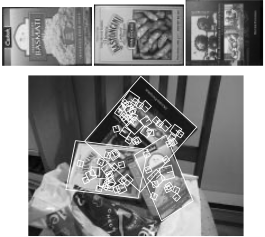
\includegraphics[scale=1.00]{figures/sift_img.png}
	\captionof{figure}{Exemplo de Detecção utilizando SIFT}
	\label{fig:1}
\end{center}

\subsection[SURF]{Speeded Up Robust Feature}

Speeded Up Robust Feature (SURF) é uma técnica bastante próxima
de SIFT\ref{sift}, contudo tem a vantagem de ser mais robusta às transformações que se pode
fazer às imagens conseguindo também, ao mesmo tempo, aumentar a performance
e a repitibilidade da detecção nas imagens \cite{citeulike:973069}.

As melhorias enunciadas são conseguidas através da escolha cuidadosa
dos pontos característicos de um objecto. Esta escolha é feita
utilizando o conceito de imagens integrais \cite{10.1109CVPR.2001.990517}
cujo conceito básico é que cada pixel $x$ na imagem inicial é a
soma dos valores dos pixeis no rectângulo formado pela origem da
imagem e as coordenadas do pixel actual:

\[
I_\sum(x) = \sum_{i \leq x}^{i=0} \sum_{j \leq y}^{j=0} I(i,j)
\]


A vantagem destas imagens integrais é que são necessárias apenas adições
para calcular a soma das intensidades em qualquer área rectangular vertical.

Os pontos característicos são encontrados onde o determinante de uma matriz
hessiana é máxima.


\subsection{Geometric Hashing}

O geometric hashing, tal como os métodos acima representados é uma técnica baseada
em modelos pré-existentes que visa reconhecer objectos onde são aplicadas rotações,
translações e escala \cite{1989SPIE.1095..515C}

Esta técnica tem por base também pontos característicos que são obtidos por
conjuntos de três pontos não colineares segundo os quais os outros são achados. 
Desta forma os seus pontos característicos não variam de acordo com as 
transformações que possam ser aplicadas aos objectos.

%\subsection{Conditional Random Fields}


\subsection{RANSAC}

RANSAC\cite{Fischler:1981:RSC:358669.358692}, um acrónimo de \emph{RANdom SAmple Consensus},
é um algoritmo que permite extrair, através de um conjunto de dados, os parâmetros
do modelo matemático que compõe as características aproximadas do objecto. Este algoritmo 
funciona de forma iterativa, sendo que a cada iteração melhora a qualidade dos parâmetros extraídos.

Este método representa uma evolução significativa dos métodos mínimos quadrados 
\footnote{devo referir o método dos mínimos quadrados antes?} visto ser
permeável a desvio dos dados sem que estes afectem a qualidade da modelação matemática.
Como se pode ver na figura \ref{fig:ransac_vs_lsq} o método \emph{RANSAC} será um método
melhor para uma situação real onde os dados têm muito ruído.


\begin{center}
	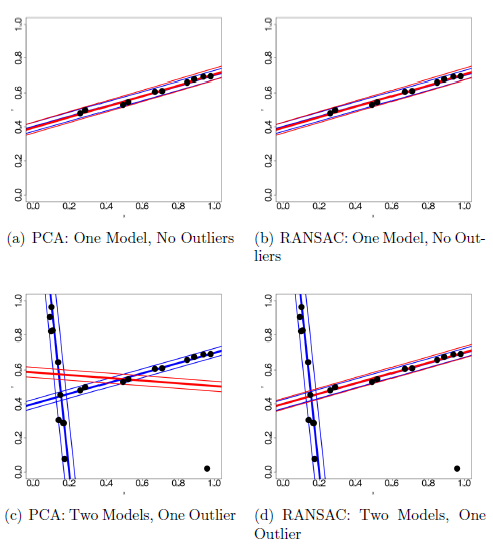
\includegraphics[width=0.80\textwidth]{figures/least_squares_vs_ransac.png}
	\captionof{figure}{Comparação com o método de mínimos quadrados}
	\label{fig:ransac_vs_lsq}
\end{center}



\begin{center}
	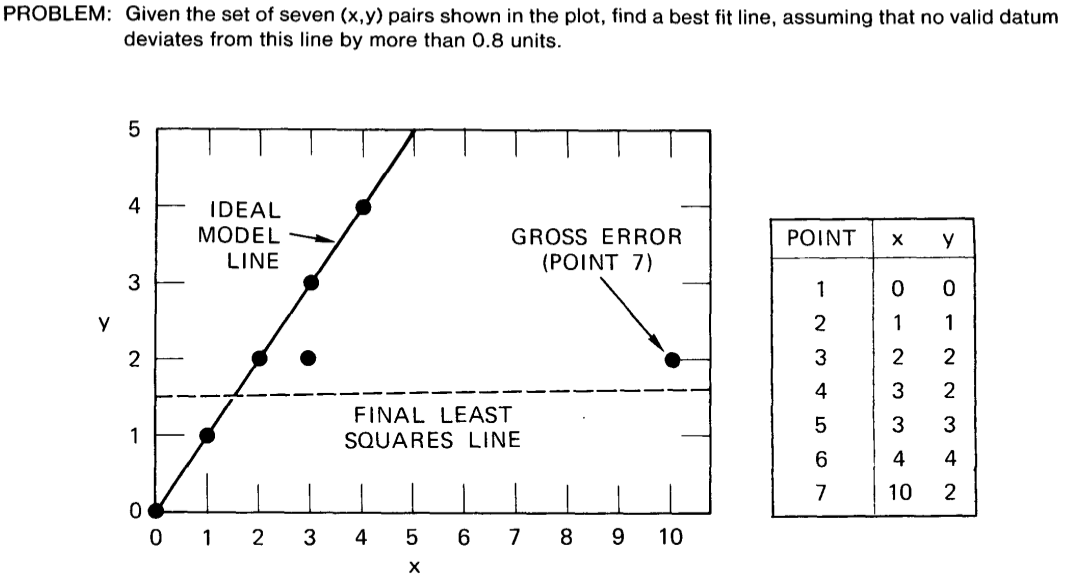
\includegraphics[width=0.80\textwidth]{figures/least_squares_shortcomings.png}
	\captionof{figure}{Exemplo de fraqueza do método de mínimos quadrados}
	\label{fig:ransac}
\end{center}


\subsection[PCL]{Point Cloud Library}

\emph{Point Cloud Library} (PCL) é um projecto \emph{opensource} desenvolvido em C++ 
cujo objectivo é disponibilizar uma ferramenta altamente optimizada para 
processar nuvens de pontos. Nuvens de pontos são a informação 3D que sensores 
como o \emph{Kinect} devolvem, que não é mais do que a nuvem dos pontos captados no espaço,
com a origem no ponto onde o sensor se encontra, também com a informação 
O projecto Point Cloud Library (PCL) \cite{Rusu_ICRA2011_PCL} permite que
através da nuvem de pontos se extraia a informação desejada, sendo que
já tem implementado um conjunto de filtros, técnicas de reconstrução de
superfícies, métodos de extracção de características 3D (por exemplo
normais às superfícies), que a tornam uma ferramenta de muito interessante para usar
a par do \emph{Kinect}.


Um exemplo de uma captura de imagem através do PCL encontra-se na imagem...


\section{Demonstradores de Robótica Autónoma}
Esta secção refere-se a demonstradores de robótica autónoma, onde são referidos
os exemplos que traduzem o que se está a fazer no âmbito de demonstradores de
robótica autónoma e que representam o estado da arte nesta área.


\subsection{DARPA: Grand challenge}
A agência norte americana DARPA (\emph{Defense Advanced Research Agency}), cujos projectos de
investigação se destinam principalmente a aplicações militares, realizou três grandes
eventos onde foram postos à prova as técnicas de condução autónoma de veículos
comerciais devidamente equipados e modificados para se poderem mover de uma forma
completamente autónoma.  

Existiram duas edições do \emph{Grand Challenge} realizadas em 2004 e 2005 que consistia
numa prova de condução autónoma em que os carros percorriam uma estrada de cerca
de 242km no deserto do \emph{Mojave}. Em 2004 nenhum dos concorrentes chegou ao final da
prova, sendo que o o robô que mais distância percorreu ficou pelos 18km, contudo em 2005

Em 2007 foi realizado um \emph{Urban Challenge} onde se aproximou as provas às condições
encontradas num ambiente urbano, ou seja, estradas com carros a circular em ambas as
vias, cruzamentos, sinalização vertical  e semáforos.

Na edição de 2007 os veículos autónomos estão equipados com um conjunto de sensores
 entre os quais se destacam LIDAR, Radares, sonares e infravermelhos. O projecto
vencedor desenvolvido pela Universidade de \emph{Carnegie Mellon} e apelidado de
 \emph{Boss} \cite{Urmson:2008:ADU:1395073.1395077} tem
18 sensores dispostos como apresentado no diagrama abaixo:

\begin{center}
	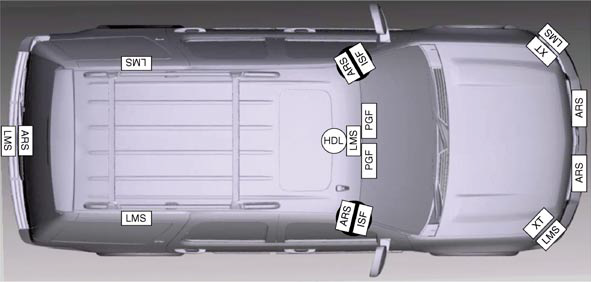
\includegraphics[width=0.80\textwidth]{figures/boss_sensors.png}
	\captionof{figure}{Sensores no Boss \cite{Urmson:2008:ADU:1395073.1395077}.}
	\label{fig:2}
\end{center}

\begin{table}
\begin{center}
\begin{tabular} { c c l }
	Sigla & Tipo de Equipamento & Modelo \\
	\hline
	APLX & GPS & Applanix POS-LV 220/420 GPS/IMU \\
	LMS & LIDAR & SICK LMS 291-S05/S14 LIDAR \\
	HDL & LIDAR & Velodyne HDL-64 LIDAR \\
	ISF & LIDAR & Continental ISF 172 LIDAR \\
	XT & LIDAR & IBEO Alasca XT LIDAR \\
	ARS & RADAR & Continental ARS 300 Radar \\
	PGF & Câmara HDR & Point Grey Firefly \\
	\hline
\end{tabular}
	\caption{Listagem dos sensores do \emph{Boss}}
	\label{boss_sensor}
\end{center}
\end{table}

Sendo que os códigos dos sensores correspondem ao indicado na tabela ~\ref{boss_sensor}
pode-se concluir, que os sensores LIDAR são um excelente sensor para ajudar no reconhecimento
de objectos no mundo, tal como para mapear o ambiente do robô para se poder orientar de uma eficaz.


\subsection{Festival Nacional de Robótica}

O festival nacional de robótica é um evento organizado anualmente pela sociedade
portuguesa de robótica em cidades diferentes onde, além de um encontro de científico
onde investigadores de robótica de todo o mundo discutem e apresentam os trabalhos
que estão a desenvolver, são realizadas várias competições e demonstrações de robótica.

As competições que se realizam são as seguintes:
\begin{itemize}
\item    Busca e Salvamento Júnior RoboCup
\item    Dança Júnior RoboCup
\item    Futebol Robótico Júnior RoboCup
\item    Condução Autónoma
\item    Liga INFAIMON Futebol Robótico Médio RoboCup
\item    FreeBots
\item    Robot@Factory
\item    Equipas
\item    Qualificações para o RoboCup
\end{itemize}

Destas competições, a mais relevante para o trabalho a ser desenvolvido no 
âmbito desta dissertação é a de Competição Autónoma, onde um robô totalmente 
autónomo tem de navegar numa pista em oito que tem as características apresentadas:

\begin{center}
	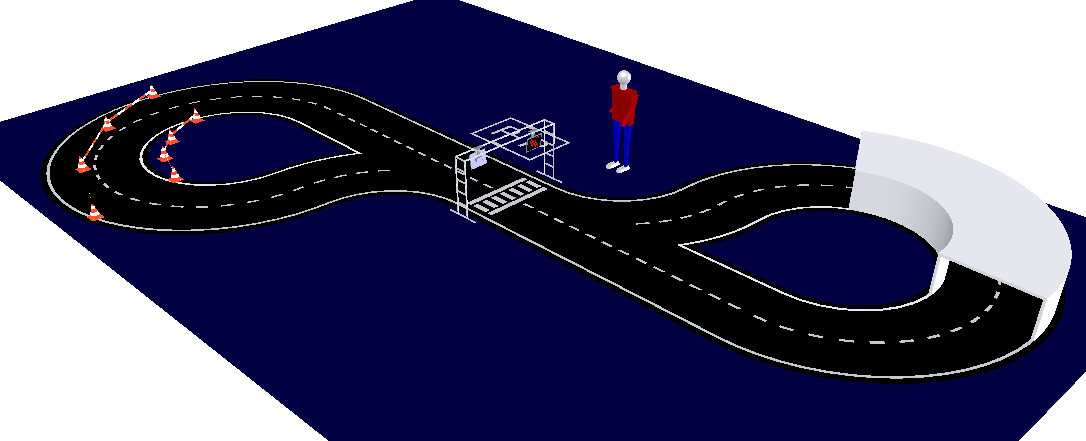
\includegraphics[width=1.00\textwidth]{figures/ca_pista.png}
	\captionof{figure}{Pista de Condução Autónoma no Festival Nacional de Robótica}
	\label{fig:3}
\end{center}

O objectivo é o robô percorrer a pista circulando pela faixa da direita, seguindo
as indicações no sinais verticais que se situam à beira da pista e os semáforos,
e evitar os obstáculos que sinalizam obras no percurso.


\subsection{MINERVA}
O minerva é um robô autónomo desenvolvido na universidade Carnegie Mellon, para
fazer de robô guia no museu smithsonian para a exposição de história natural que
esteve em exibição no periodo de 25 de Agosto a 5 de Setembro de 1998.

\begin{center}
	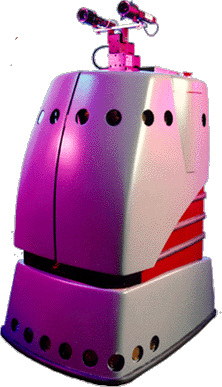
\includegraphics[width=0.20\textwidth]{figures/minerva.png}
	\captionof{figure}{MINERVA - Robô guia do museu Smithsonian}
	\label{fig:4}
\end{center}

Este robô era totalmente autónomo a partir do momento em que fazia uma volta de
aprendizagem, em que era guiado pelo percurso que lhe estava destinado. Estando
a aprendizagem concluída, o robô orientava-se pelo resultado da sua aprendizagem,
e por alguns sensores, nomeadamente para se desviar dos visitantes e de obstáculos,
uma câmara para detectar marcadores no tecto do museu para se conseguir localizar.
Além de guiar os visitantes pelo percurso este robô também interagia com os mesmos,
respondendo a perguntas e apresentando a exposição.

\subsection{CleanRob}

O CleanRob é um projecto que começou a ser desenvolvido na Faculdade de Engenharia da 
Universidade do Porto em 2004, no no contexto do Departamento de Engenharia
Electrotécnica e de Computadores. Este robô foi desenvolvido por alunos de modo a
envolver alunos no desenvolvimento de projectos académicos com maior aplicação prática
tirando partido de técnicas que representam o estado da arte na robótica.

Este robô utiliza um conjunto de câmaras e sonares PSD para fazer a sua localização,
de modo a limpar corredores do departamento de Engenharia Electrotécnica.

\begin{center}
	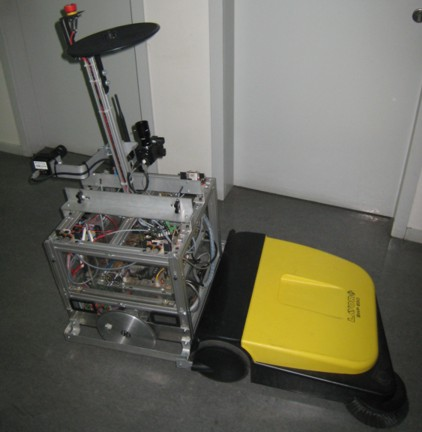
\includegraphics[width=0.40\textwidth]{figures/clean_rob.jpeg}
	\captionof{figure}{CleanRob}
	\label{fig:6}
\end{center}


\section{Planeamento}

O desenrolar desta dissertação será de Setembro a meados de Fevereiro de 2012, sendo
que diferentes tarefas estão agendadas para diferentes fases. As tarefas para a realização
desta dissertação com sucesso são as seguintes:
\begin{itemize}
\item Estado da Arte;
\item Arquitectura de Sistema;
\item Reconhecimento de Objectos:
\begin{itemize}
\item Cilindros;
\item Esferas;
\item Paralelepípedos.
\item Mesas;
\end{itemize}
\item Testes ao Sistema;
\item Refinamentos;
\item Escrita da Dissertação.
\end{itemize}

Estas tarefas terão um tempo atribuído para serem cumpridas, que seguirá o que está estipulado no
diagrama ~\ref{fig:7}.

\begin{center}
	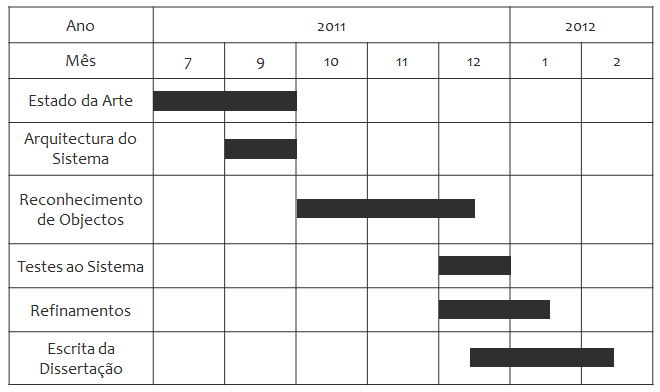
\includegraphics[width=0.70\textwidth]{figures/diss_timetable.PNG}
	\captionof{figure}{Planeamento de Tarefas}
	\label{fig:7}
\end{center}

\section{Resumo}

No que diz respeito a detecção de objectos, existem vários algoritmos bastante robustos e
eficazes na detecção de objectos, contudo são muito voltados para reconhecimento em imagens RGB
e não tanto baseados em conjuntos de dados 3D e além disso exigem uma fase de aprendizagem.

Os demonstradores autónomos que existem no momento já são bastante completos, considere-se
como exemplo o \emph{Boss} que navega em ambiente bastante próximo do urbano com proeza,
estando cada vez mais próximo de um cenário onde condução autónoma nas cidades poderia ser
uma realidade e até mesmo uma mais-valia em termos de segurança. É de assinalar também os esforços
nas competições de robôs em escalas menores pois com menos recursos e menor escala consegue-se
testar técnicas inovadoras com soluções menos dispendiosas obtendo-se resultados igualmente
impressionantes.

